\documentclass{standalone}
\usepackage{tikz}
\usepackage{tkz-graph}
\usepackage{tkz-berge}

\begin{document}

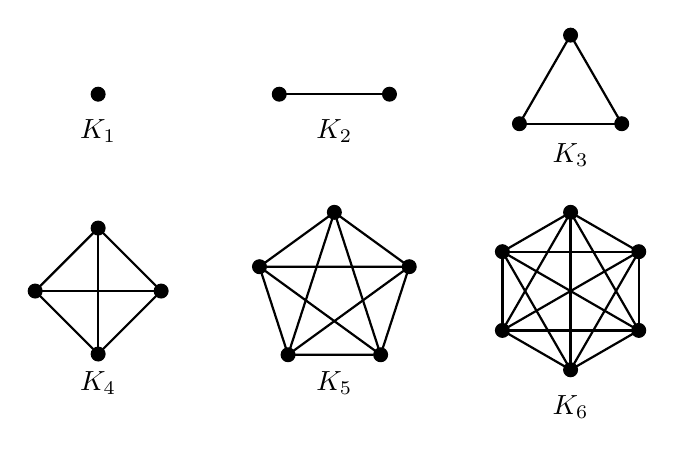
\begin{tikzpicture}
  \GraphInit[vstyle=Simple]
  \tikzset{VertexStyle/.style = {
  shape = circle,
  fill = black,
  inner sep = 0pt,
  outer sep = 0pt,
  minimum size = 5pt,
  draw}}
  \SetVertexMath
  \begin{scope}[yshift=2.5cm, rotate=90+((360/1)*3)]
    \grComplete[RA=0]{1}
  \end{scope}
  \begin{scope}[yshift=2.5cm, xshift=3cm, rotate=0]
    \grComplete[RA=0.7]{2}
  \end{scope}
  \begin{scope}[yshift=2.5cm, xshift=6cm, rotate=90+((360/3)*3)]
    \grComplete[RA=0.75]{3}
  \end{scope}
  \begin{scope}[yshift=0cm, rotate=90+((360/8)*4)]
    \grComplete[RA=0.8]{4}
  \end{scope}
  \begin{scope}[yshift=0cm, xshift=3cm, rotate=90+((360/5)*3)]
    \grComplete[RA=1]{5}
  \end{scope}
  \begin{scope}[yshift=0cm, xshift=6cm, rotate=90+((360/6)*3)]
    \grComplete[RA=1]{6}
  \end{scope}
  \draw (0, 2.3) node [below]{$K_1$};
  \draw (3, 2.3) node [below]{$K_2$};
  \draw (6, 2.0) node [below]{$K_3$};
  \draw (0,-0.9) node [below]{$K_4$};
  \draw (3,-0.9) node [below]{$K_5$};
  \draw (6,-1.2) node [below]{$K_6$};
\end{tikzpicture}

\end{document}
